\documentclass[12pt, letterpaper]{article}
\usepackage[top=1in, bottom=1in, left=1.5in, right=1.5in]{geometry}
\usepackage{amsmath}
\usepackage{amsfonts}
\usepackage{natbib}
\usepackage{mathtools}
\usepackage{amssymb}
\usepackage{fullpage}
\usepackage{listings}
\usepackage{float}
\usepackage{natbib}
\usepackage{url}
\usepackage[clockwise]{rotating}
\usepackage{caption}
\usepackage{graphicx}
\let\oldtabular\tabular
\renewcommand{\tabular}{\footnotesize\oldtabular}
%\newcommand\Fontvi{\fontsize{8}{7.2}\selectfont}

\lstset{language=R}
%\setlength{\textwidth}{150mm}
\linespread{1.6}
\bibpunct{(}{)}{;}{a}{,}{,}

\begin{document}
\title{Earnings Forecasts from Firm-Level Regressions: Implications for Research and Practice}
\author{Reginald Edwards\footnote{Ross School of Business, University of 
Michigan (\texttt{reggie@umich.edu}).}}
\date{This Draft: 1 September 2014}
\maketitle

\begin{abstract} 

%Short motivation. Short research question. Short contribution. Short conclusion.
Analyst 
forecasts are used in research  on valuation, cost of capital, and more. In this paper I deconstruct
this supposed advantage of analysts over statistical forecasts. I develop and evaluate a novel
statistical forecasting framework for earnings. I reinterpret and reevaluate estimates of firms' 
implied cost of capital and market-level risk premia that rely on analyst forecasts by using a 
statistical forecast. I examine if the main strength of the purported superioty of analyst forecasts
is concentrated in the period prior to the passage of Regulation Fair Disclosure (Reg FD). 
My work posits a model of earnings that has many of the 
desirable properties of analyst forecasts, but less bias and is applicable to more firms and years.
This model is thus more useful to both researchers and practitioners.

\end{abstract}

\section{Introduction}


\section{Literature Review}

\subsection{Statistical Earnings Forecasts}


\subsection{Analysts' Earnings Forecasts}


\subsection{Implications for Implied Cost of Capital Estimates}

\subsection{Implications for the Equity Risk Premium}


\section{Research Design}
\subsection{Earnings Forecasts}

%\subsection{Implied Cost of Capital}

%\subsection{Market Equity Premium}

%\subsection{Trading Strategy}

\section{Data}
\subsection{Data Overview}
%A correlation matrix for the variables of interest are given in Table \ref{corr-matrix}.
% Table 1



%\input{../tables/corr-matrix2.tex}


\subsection{Sample Selection}

\section{Results}
\subsection{Univariate Results}

In the ``univariate'' equation above, $X_{t-1}$ is the lagged observation of a predictor. Table 
\ref{univariate-stats-eps} below shows summary statistics for the firm-level univariate 
regressions. 

Table \ref{univariate-stats-eps-rsquared} shows summary statistics for $R^2$ values of
these regressions. Predictors with high incremental $R^2$ values may be predictive in subsequent 
out-of-sample tests and the values may serve to limit the set of predictors. In particular, the 
lower in-sample explanatory power of $Accruals$ compared with $\Delta AP$ and $\Delta AR$ serve as
partial motivation for the former to be replaced by the latter two in the multivariate model.

\subsection{Earnings Forecasts}
To assess how the model performs by target year (the target firm's fiscal year end in which 
earnings will be announced), 
I compute mean squared prediction errors (MSPE) for all target years. The 
results in Table \ref{spe-by-year-table-fy1} show MSPE by target year for the model, mean analyst 
forecast, and median analyst forecast. All three estimates do extremely poorly during the dotcom
bubble bursting period. \footnote{MSPE comparisons for two-year-ahead and three-year-ahead 
forecasts have been omitted.}
%% latex table generated in R 3.0.2 by xtable 1.7-1 package
% Sun Aug 31 12:06:31 2014
\begin{table}[H]
\centering
\begin{tabular}{lcccc}
  \hline
Year & Model & MEANEST & MEDEST \\ 
  \hline
1993 & 0.036 & 1.369 & 1.369 \\ 
1996 & 0.040 & 0.102 & 0.102 \\ 
1997 & 0.055 & 1.640 & 1.570 \\ 
1998 & 4.306 & 0.268 & 0.385 \\ 
1999 & 0.411 & 6.683 & 6.684 \\ 
2000 & 0.036 & 0.069 & 0.076 \\ 
2001 & 0.374 & 0.027 & 0.022 \\ 
2002 & 0.099 & 0.119 & 0.119 \\ 
2003 & 0.369 & 0.264 & 0.281 \\ 
2004 & 0.094 & 0.585 & 0.680 \\ 
2005 & 1.737 & 1.892 & 1.917 \\ 
2006 & 1.431 & 1.179 & 1.153 \\ 
2007 & 0.547 & 1.716 & 1.670 \\ 
2008 & 1.414 & 0.726 & 0.723 \\ 
2009 & 3.686 & 3.574 & 3.627 \\ 
2010 & 1.720 & 1.559 & 1.570 \\ 
2011 & 2.373 & 1.601 & 1.541 \\ 
2012 & 4.759 & 4.189 & 4.212 \\ 
   \hline
\end{tabular}
\captionsetup{width=5.5in, font=footnotesize}
\caption{Mean squared prediction error of model forecast, mean analyst (MEANEST) forecast, and 
median analyst forecast (MEDEST). Forecasts are of two-year-ahead earnings.} 
\label{spe-by-year-table-fy2}
\end{table}

%% latex table generated in R 3.0.2 by xtable 1.7-1 package
% Sun Aug 31 12:30:41 2014
\begin{table}[H]
\centering
\begin{tabular}{lcccc}
  \hline
Year & Model & MEANEST & MEDEST \\ 
  \hline
1993 & 0.036 & 0.941 & 0.941 \\ 
1996 & 0.040 & 4.622 & 4.622 \\ 
1997 & 0.055 & 0.944 & 0.944 \\ 
1998 & 1.340 & 3.728 & 3.728 \\ 
1999 & 0.278 & 0.535 & 0.535 \\ 
2000 & 12.362 & 0.029 & 0.020 \\ 
2001 & 0.374 & 0.029 & 0.029 \\ 
2002 & 0.168 & 0.053 & 0.053 \\ 
2003 & 0.369 & 1.205 & 1.205 \\ 
2004 & 0.472 & 1.195 & 1.195 \\ 
2005 & 0.830 & 3.468 & 3.468 \\ 
2006 & 1.448 & 1.217 & 1.217 \\ 
2007 & 0.605 & 2.388 & 2.167 \\ 
2008 & 1.473 & 1.084 & 1.107 \\ 
2009 & 2.823 & 4.898 & 4.560 \\ 
2010 & 1.890 & 1.672 & 1.629 \\ 
2011 & 2.075 & 3.351 & 3.082 \\ 
2012 & 4.452 & 4.707 & 4.711 \\ 
   \hline
\end{tabular}
\captionsetup{width=5.5in, font=footnotesize}
\caption{Mean squared prediction error of model forecast, mean analyst (MEANEST) forecast, and 
median analyst forecast (MEDEST). Forecasts are of three-year-ahead earnings.} 
\label{spe-by-year-table-fy3}
\end{table}


%  \begin{figure}[H]
%  \begin{center}
%    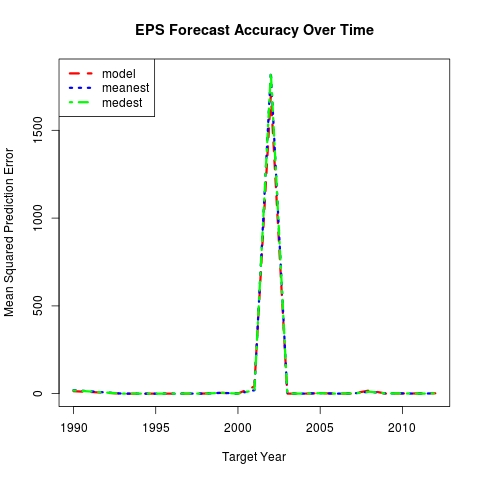
\includegraphics[height=4in]{../graphics/eps-by-year-fy1.jpeg}
%    \caption{Mean squared prediction error for model and consensus forecasts by target forecast year.}
%    \label{spe-by-year-graph-fy1}
%  \end{center}
%  \end{figure}
  
\textbf{Does private information help analyst forecasts?} Table \ref{evaluation-regfd} presents
comparisons of the model's accuracy before and after implementation of Regulation Fair Disclosure. 
As noted in prior literature (e.g. \cite{gintschelmarkov2004}) analyst forecasts are worse in the 
post-Reg FD period. The performance of the model forecasts does not change in any consistent way
pre- and post-Reg FD.\footnote{In this section and all others, ``consensus'' forecasts refer to the
mean analyst estimate. Results with median analyst estimates are qualitatively similar.}


\textbf{The effects of \emph{ex ante} uncertainty on forecasts.} Table \ref{evaluation-dispersion}
presents comparisons of the accuracy of model and consensus forecasts during information 
environments characterized by high and low uncertainty. Both the model and analyst forecasts 
perform better during periods characterized by low analyst dispersion.\footnote{Dispersion is 
measured as the standard deviation of analyst forecasts. High (low) dispersion periods are those
with a standard deviation above (below) the median. Results are not sensitive to choice of 
percentile.} For the one-year-ahead forecasts, the model performs relatively better than consensus
forecasts.

%\subsection{Implied Cost of Capital}

%\subsection{Market Equity Premium}

\subsection{Earnings Forecasts as Trading Signals}
Most studies that compare time series forecasts to analyst forecasts use a loss function (evaluation
criterion) that is some form of relative prediction error or bias. To better quantify the 
significance of divergence between the consensus forecasts of earnings and the model forecast, I 
examine the returns
to an investor who uses the divergence in analyst and model forecasts as a signal. As a first step,
I calculate buy and hold returns ($BAHR$) for each firm from the forecast date to one month and, 
separately,
two months after the target date (i.e., the date at which forecasted earnings are revealed.) I do 
this for all forecasts (one-, two-, and three-year-ahead forecasts.) I then compute the divergence
between the model forecasts and the consensus forecast, $DIFF$, as the model forecast less the 
consensus forecast. $DIFF$ is calculated for each forecast horizon. For each forecast target and 
returns horizon I run a regression of the form

\begin{equation}
BAHR_{t+\tau} = \alpha_{0} + \alpha_{1}DIFF_{i} + \varepsilon.
\end{equation}

Table \ref{evaluation-bahr} shows the coefficient and p-values from each of these regressions. 
For the forecasts of FY1 earnings, buy-and-hold returns are positively and statistically 
significantly related to the degree of 
divergence between model forecasts and consensus analyst forecasts. Note, however, that
returns have not been adjusted for standard asset pricign risk factors.
\\

Next, I rank and group each forecast into deciles by the level of divergence. As Figures
\ref{bahr-diff-decile} and \ref{bahr-diff-decile2} show, the buy-and-hold returns over the forecast
horizon for the forecast of FY1 earnings is increasing in the level of divergence between the model
and the consensus forecast. This indicates that the stock returns of firms for which the model
forecasts higher earnings than analysts are higher than those for which analysts are more optimistic
than the model suggests.
\\

  
\section{Conclusions and Extensions}


\bibliographystyle{aea}
\bibliography{articles}
\newpage
\section*{Appendix: Tables and Figures}
% latex table generated in R 3.0.2 by xtable 1.7-3 package
% Tue Aug 26 15:23:31 2014
\begin{table}[H]
\centering
\begin{tabular}{lrrrrr}
  \hline
 & mean & med & min & max & stdev \\ 
  \hline
EPS & 1.504 & 1.165 & -21.690 & 89.610 & 2.103 \\ 
  EPS Growth & 0.126 & 0.121 & -246.500 & 768.000 & 8.127 \\ 
  Total Assets & 8858.471 & 2038.377 & 48.195 & 797769.000 & 30477.603 \\ 
  Accruals & -0.030 & -0.037 & -1.013 & 2.832 & 0.121 \\ 
  Dividends & 0.541 & 0.274 & 0.000 & 51.403 & 0.929 \\ 
  Dividend Payer & 0.203 & 0.000 & 0.000 & 1.000 & 0.402 \\ 
  Negative Earnings & 0.056 & 0.000 & 0.000 & 1.000 & 0.229 \\ 
  Delta Price & 0.083 & 0.038 & -2.674 & 14.366 & 0.486 \\ 
  return & -0.003 & 0.038 & -3.501 & 2.732 & 0.422 \\ 
  PE Ratio & 59.508 & 24.157 & -110000.000 & 151250.000 & 1635.234 \\ 
  GDP & 0.048 & 0.049 & -0.032 & 0.124 & 0.023 \\ 
  ROE & 0.482 & 0.147 & -282.640 & 5822.013 & 44.669 \\ 
  Unemployment & 0.062 & 0.056 & 0.038 & 0.108 & 0.017 \\ 
  Inflation (PPI) & 0.003 & 0.003 & -0.053 & 0.030 & 0.011 \\ 
  Sales & 8096.594 & 1975.248 & -7.237 & 470171.000 & 25083.807 \\ 
  AR & 1497.423 & 258.700 & 0.000 & 418777.000 & 10231.124 \\ 
  AP & 783.347 & 127.400 & 0.000 & 149813.000 & 3446.179 \\ 
  Age & 16.396 & 15.000 & 5.000 & 32.000 & 7.977 \\ 
 $\Delta Sales$ & 832.864 & 154.138 & -295570.000 & 368056.000 & 7283.693 \\ 
  $\Delta AR$ & 128.839 & 18.461 & -45714.199 & 99095.000 & 1780.134 \\ 
  $\Delta AP$ & 76.889 & 8.921 & -83588.000 & 71555.000 & 1149.442 \\ 
   \hline
\end{tabular}
\captionsetup{width=4in, font=footnotesize}
\caption{Summary statistics of EPS and independent variables. $Age$ is number of years company is in the sample.}
\label{summary-stats}
\end{table}
\newpage
% latex table generated in R 3.1.1 by xtable 1.7-4 package
% Thu Feb 26 16:52:22 2015
\begin{table}[ht]
\centering
\begin{tabular}{rrrrrr}
  \hline
 & mean & med & min & max & stdev \\ 
  \hline
$EPS_{t-1}$ & 0.8027 & 0.8753 & -0.1915 & 1.6592 & 0.2938 \\ 
assets & 0.0408 & 0.0211 & -0.2675 & 1.2235 & 0.1008 \\ 
  Accruals & 1.1515 & 0.1889 & -27.7192 & 51.6659 & 5.7370 \\ 
  Dividends & -1.9528 & -0.0001 & -868.1679 & 101.1100 & 44.6254 \\ 
  Negative Earnings & 0.2092 & 0.1332 & -4.6542 & 5.7750 & 1.4040 \\ 
  $\Delta Price$ & 0.5412 & 0.2741 & -1.0112 & 29.5364 & 1.5372 \\ 
  return & 0.5667 & 0.2829 & -1.0074 & 31.0738 & 1.6127 \\ 
  PE Ratio & -0.0036 & -0.0004 & -0.2647 & 0.0760 & 0.0213 \\ 
  GDP & 3.4401 & 1.8823 & -122.6991 & 64.2745 & 12.9067 \\ 
  ROE & 2.0801 & 0.9929 & -6.2682 & 24.3831 & 3.4486 \\ 
  Unemployment & -1.2504 & 0.1596 & -176.6090 & 97.6023 & 21.2597 \\ 
  Inflation (PPI) & 10.6295 & 4.8897 & -162.8660 & 168.6141 & 27.7419 \\ 
  Sales & 0.5747 & 0.3485 & -3.3250 & 9.0993 & 1.1306 \\ 
  AR & 0.0681 & 0.0322 & -0.3495 & 1.7380 & 0.1476 \\ 
  AP & 0.0757 & 0.0435 & -0.3640 & 1.6566 & 0.1532 \\ 
  $\Delta Sales$ & 0.0004 & 0.0001 & -0.0022 & 0.0093 & 0.0009 \\ 
  $\Delta AR$ & 0.0018 & 0.0005 & -0.0268 & 0.1659 & 0.0091 \\ 
  $\Delta AP$ & 0.0023 & 0.0008 & -0.0631 & 0.0523 & 0.0086 \\ 
   \hline
\end{tabular}
\caption{Coefficients from regressions of the form $EPS_{t} = \alpha_0 + \alpha_{1}EPS_{t} + \alpha_{2}X_{t-1} +\varepsilon.$} 
\label{univariate-stats-eps-rsquared}
\end{table}\newpage
% latex table generated in R 3.0.2 by xtable 1.7-3 package
% Thu Aug 28 12:40:48 2014
\begin{table}[H]
\centering
\begin{tabular}{rrrrrr}
  \hline
 & mean & med & min & max & stdev \\ 
  \hline
$EPS_{t-1}$ & 0.6226 & 0.6972 & 0.0002 & 0.9981 & 0.3130 \\ 
assets & 0.6440 & 0.7110 & 0.0013 & 0.9982 & 0.2984 \\ 
  Accruals & 0.6491 & 0.7069 & 0.0068 & 0.9983 & 0.2849 \\ 
  Dividends & 0.6490 & 0.7168 & 0.0063 & 0.9984 & 0.2962 \\ 
  Negative Earnings & 0.6353 & 0.7079 & 0.0006 & 0.9981 & 0.2995 \\ 
  $\Delta Price$ & 0.6901 & 0.7469 & 0.0224 & 0.9981 & 0.2624 \\ 
  return & 0.6957 & 0.7549 & 0.0179 & 0.9981 & 0.2588 \\ 
  PE Ratio & 0.6431 & 0.7152 & 0.0128 & 0.9982 & 0.2961 \\ 
  GDP & 0.6578 & 0.7366 & 0.0062 & 0.9983 & 0.2927 \\ 
  ROE & 0.7294 & 0.7957 & 0.0045 & 0.9982 & 0.2406 \\ 
  Unemployment & 0.6618 & 0.7358 & 0.0010 & 0.9984 & 0.2877 \\ 
  Inflation (PPI) & 0.6647 & 0.7364 & 0.0296 & 0.9982 & 0.2829 \\ 
  Sales & 0.6870 & 0.7596 & 0.0009 & 0.9982 & 0.2743 \\ 
  AR & 0.6497 & 0.7148 & 0.0010 & 0.9983 & 0.2931 \\ 
  AP & 0.6514 & 0.7234 & 0.0079 & 0.9982 & 0.2932 \\ 
$\Delta Sales$ & 0.7089 & 0.7838 & 0.0047 & 0.9984 & 0.2684 \\ 
$\Delta AR$ & 0.6744 & 0.7403 & 0.0110 & 0.9983 & 0.2781 \\ 
$\Delta AP$ & 0.6690 & 0.7364 & 0.0027 & 0.9981 & 0.2822 \\ 
   \hline
\end{tabular}
\captionsetup{width=4in, font=footnotesize}
\caption{$R^2$ values from regressions of the form $EPS_{t} = \alpha_0 + \alpha_{1}EPS_{t} + \alpha_{2}X_{t-1} +\varepsilon.$} 
\label{univariate-stats-eps-rsquared}
\end{table}\newpage
% latex table generated in R 3.0.2 by xtable 1.7-3 package
% Sun Aug 31 11:31:11 2014
\begin{table}[H]
\centering
\begin{tabular}{rrrr}
  \hline
Year & Model & MEANEST & MEDEST \\ 
  \hline
1990 & 14.440 & 20.250 & 18.662 \\ 
1993 & 0.116 & 0.152 & 0.176 \\ 
1994 & 0.096 & 0.137 & 0.137 \\ 
1995 & 0.166 & 0.037 & 0.031 \\ 
1996 & 0.122 & 0.002 & 0.000 \\ 
1997 & 0.180 & 0.554 & 0.606 \\ 
1998 & 1.018 & 0.196 & 0.201 \\ 
1999 & 4.547 & 5.233 & 5.126 \\ 
2000 & 0.542 & 0.379 & 0.324 \\ 
2001 & 41.042 & 19.687 & 19.687 \\ 
2002 & 1701.955 & 1832.864 & 1828.333 \\ 
2003 & 0.152 & 0.151 & 0.148 \\ 
2004 & 0.263 & 0.365 & 0.359 \\ 
2005 & 2.929 & 2.737 & 2.749 \\ 
2006 & 0.593 & 0.211 & 0.209 \\ 
2007 & 0.771 & 1.316 & 1.389 \\ 
2008 & 18.404 & 11.094 & 11.298 \\ 
2009 & 0.592 & 1.357 & 1.303 \\ 
2010 & 1.658 & 1.379 & 1.381 \\ 
2011 & 1.016 & 0.367 & 0.378 \\ 
2012 & 2.357 & 1.612 & 1.618 \\ 
   \hline
\end{tabular}
\captionsetup{width=3in, font=footnotesize}
\caption{Mean squared prediction error of model forecast, mean analyst (MEANEST) forecast, and 
median analyst forecast (MEDEST). Forecasts are of one-year-ahead earnings.} 
\label{spe-by-year-table-fy1}
\end{table}
\newpage
\begin{table}[H]
\centering
\begin{tabular}{l | c c | c c}
  \hline
&  \multicolumn{2}{| c}{Pre-Reg FD} &  \multicolumn{2}{| c}{Post-Reg FD} \\
% & Pre-Reg FD & & Post-Reg FD & \\ 
  \hline
 Forecast horizon & Model & Consensus & Model & Consensus \\ 
  \hline
1-Year Ahead & 2.365 & 2.466 & 27.479 &28.159 \\ 
2-Year Ahead & 2.255 & 1.905 & 4.163 & 3.672 \\ 
3-Year Ahead & 0.732 & 2.574 & 3.889 & 4.256 \\ 
   \hline
\end{tabular}
\captionsetup{width=4in, font=footnotesize}
\caption{Mean squared prediction error comparison of ``model'' and ``consensus'' earnings forecasts.}
\label{evaluation-regfd}
\end{table}
\newpage
\begin{table}[H]
\centering
\begin{tabular}{l | c c | c c}
  \hline
&  \multicolumn{2}{| c}{Low Dispersion} &  \multicolumn{2}{| c}{High Dispersion} \\
  \hline
 Forecast horizon & Model & Consensus & Model & Consensus \\ 
  \hline
1-Year Ahead & 1.45 & 0.774 &90.436 & 94.511 \\ 
2-Year Ahead & 8.133 & 7.853 & 0.874 & 0.371 \\ 
3-Year Ahead & 1.409 & 0.860 & 5.155 & 4.986  \\ 
   \hline
\end{tabular}
\captionsetup{width=4in, font=footnotesize}
\caption{Mean squared prediction error comparison of ``model'' and ``consensus'' earnings forecasts.}
\label{evaluation-dispersion}
\end{table}
\newpage
\begin{table}[H]
\centering
\begin{tabular}{l | c c | c c}
  \hline
&  \multicolumn{2}{| c}{BAHR $\tau+1$ month} &  \multicolumn{2}{| c}{BAHR $\tau+2$ months}  \\
  \hline
 Forecast horizon, $\tau$ & Coeff. & \emph{P-Value} &  Coeff. & \emph{P-Value}  \\ 
  \hline
1-Year Ahead & 0.06825** & 0.0334 & 0.06903** & 0.0329 \\ 
%1-Year Ahead & 1.706 & 1.230 & -11.060 & 38.150 \\ 
2-Year Ahead & 0.02169 & 0.344 & 0.02610 & 0.259 \\ 
%2-Year Ahead & 1.706 & 1.230 & -11.060 & 38.150 \\ 
3-Year Ahead & -0.02812 & 0.216 & -0.02903 & 0.205 \\ 
%3-Year Ahead & 1.706 & 1.230 & -11.060 & 38.150 \\ 
   \hline
\end{tabular}
\captionsetup{width=4in, font=footnotesize}
\caption{Buy-and-hold returns for FY1 ($\tau=12$), FY2 ($\tau=24$), and FY3 ($\tau=36$) 
forecasts. Return horizons are one month and two months after the forecast target date.}
\label{evaluation-bahr}
\end{table}
\newpage

  \begin{figure}[H]
  \begin{center}
    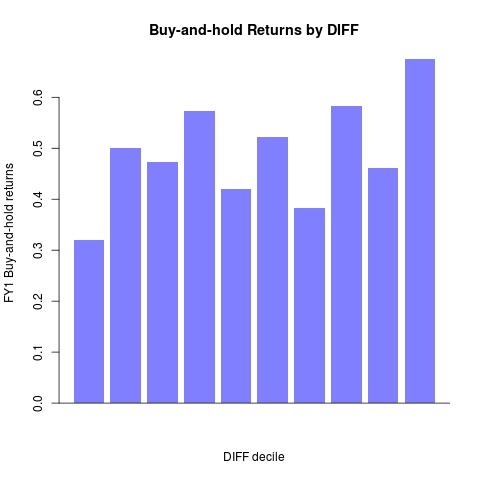
\includegraphics[height=4in]{../graphics/bahr-diff-decile.jpeg}
    \captionsetup{width=4in, font=footnotesize}
    \caption{Buy-and-hold returns by $DIFF$ decile for one-year-ahead model. $DIFF$ is the model 
    forecast of earnings less the consensus forecast.}
    \label{bahr-diff-decile}
  \end{center}
  \end{figure}

  \begin{figure}[H]
  \begin{center}
    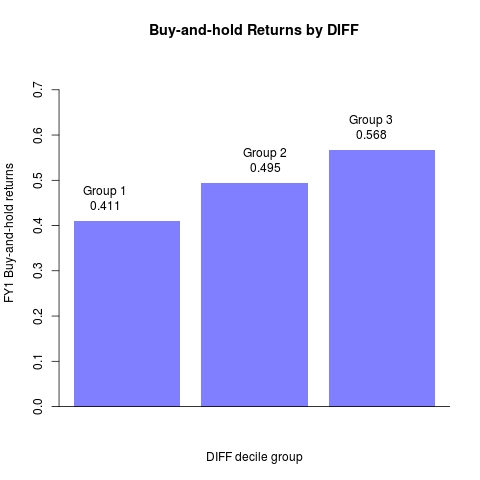
\includegraphics[height=4in]{../graphics/bahr-diff-decile2.jpeg}
    \captionsetup{width=4in, font=footnotesize}
    \caption{Buy-and-hold returns by $DIFF$ decile for one-year-ahead model. $DIFF$ is the model 
    forecast of earnings less the consensus forecast. Group 1: first and second decile. Group 3: 
    ninth and 10th deciles.}
    \label{bahr-diff-decile2}
  \end{center}
  \end{figure}
\end{document}
